\documentclass[a4paper,titlepage,12pt]{article}
\usepackage[utf8]{inputenc} %Make sure all UTF8 characters work in the document
\usepackage{graphicx}
\usepackage{titling}
\usepackage{tabularx}
\usepackage{longtable}
\usepackage[yyyymmdd]{datetime}
\usepackage[figurename=Figur]{caption}
\usepackage{booktabs}
\usepackage[parfill]{parskip}
\usepackage{xcolor}
\usepackage{listings}
\usepackage{subcaption}

\lstdefinestyle{linux}
{
	backgroundcolor=\color{black},
	basicstyle=\scriptsize\color{white}\ttfamily
}

%Set page size
\usepackage{geometry}
\geometry{margin=3cm}

\renewcommand{\dateseparator}{-}
\renewcommand{\contentsname}{Innehållsförteckning}
\renewcommand{\tablename}{Tabell}


\usepackage{color}

\usepackage[colorinlistoftodos,prependcaption,textsize=tiny]{todonotes}

\definecolor{dkgreen}{rgb}{0,0.6,0}
\definecolor{gray}{rgb}{0.5,0.5,0.5}
\definecolor{mauve}{rgb}{0.58,0,0.82}

\lstset{frame=tb,
  language=Python,
  aboveskip=3mm,
  belowskip=3mm,
  showstringspaces=false,
  columns=flexible,
  basicstyle={\small\ttfamily},
  numbers=none,
  numberstyle=\tiny\color{gray},
  keywordstyle=\color{blue},
  commentstyle=\color{dkgreen},
  stringstyle=\color{mauve},
  breaklines=true,
  breakatwhitespace=true,
  tabsize=3
}

%%%%%%%%%%%%%%%%%%%%%%%%%%%%%%%
% Header and footer
%%%%%%%%%%%%%%%%%%%%%%%%%%%%%%%
\usepackage{fancyhdr}
\pagestyle{fancy}

\lhead{
\includegraphics[width=0.15\linewidth]{../images/logo_full.png}}
\chead{Användarmanual för sexbent robot}
\rhead{\today}
\setlength\headheight{26pt} 

\lfoot{TSEA29 -- KMM \\ Användarmanual}
\rfoot{Grupp 9 \\ LiTHe Hex}

\newcommand{\itc}{I\textsuperscript{2}C}

\pretitle{%
	\begin{center}
		\LARGE
		
\includegraphics[width=6cm]{../images/logo_full.png}\\[\bigskipamount]
}

\posttitle{\end{center}}

\begin{document}
\listoftodos
	\title{\LARGE
		\textbf{Användarmanual för sexbent robot} \\
		\vspace*{0.5\baselineskip}
		\large
		Redaktör Frans Skarman \\
		Grupp 9 \\
		\small
		\vspace*{0.5\baselineskip}
		Version 0.1}

	\date{\today}

	\maketitle
	
	\newpage

	\tableofcontents
	\newpage


	%%%%%%%%%%%%%%%%%%%%%%%%%%%%%%%%%%%%%%%%%%%%%%%%%%%%%%%%%%%%%%%%%%%%%%%%%%%%%%%%%
	%						Historik
	%%%%%%%%%%%%%%%%%%%%%%%%%%%%%%%%%%%%%%%%%%%%%%%%%%%%%%%%%%%%%%%%%%%%%%%%%%%%%%%%%

	\section*{Dokumenthistorik}
	\renewcommand*{\arraystretch}{1.4}
    \begin{longtable}[c]{ l l >{\raggedright}p{5cm} >{\raggedright}p{3cm} l }
		\textbf{Version} & \textbf{Datum} & \textbf{Utförda förändringar} 
		& \textbf{Utförda av} & \textbf{Granskad} \\ \midrule
		
		0.1 & 2016--10--20 & Första utkastet & Projektgruppen &
        Projektgruppen \\
            
	\end{longtable}

	%%%%%%%%%%%%%%%%%%%%%%%%%%%%%%%%%%%%%%%%%%%%%%%%%%%%%%%%%%%%%%%%%%%%%%%%%%%%%%%%%
	%						Inledning
	%%%%%%%%%%%%%%%%%%%%%%%%%%%%%%%%%%%%%%%%%%%%%%%%%%%%%%%%%%%%%%%%%%%%%%%%%%%%%%%%%

	\newpage

	\raggedright

	\section{Inledning}
	Detta dokument går i detalj in på konstruktionen och mjukvaran för en
    sexbent robot, med autonom och manuell styrning. Först presenteras en
    översiktlig beskrivning av robotens styrande processorer ("enheter", vilka
    kopplas till ett färdigt PhantomX AX Metal Hexapod Mark III chassi från
    TrossenRobotics). Dessa (central-, motorik- och sensorenhet), kommunikation
    mellan dessa, samt användargränssnitt specificeras sedan i större
    noggrannhet under egna avdelningar.

	%%%%%%%%%%%%%%%%%%%%%%%%%%%%%%%%%%%%%%%%%%%%%%%%%%%%%%%%%%%%%%%%%%%%%%%%%%%%%%%%%
	%						Översikt
	%%%%%%%%%%%%%%%%%%%%%%%%%%%%%%%%%%%%%%%%%%%%%%%%%%%%%%%%%%%%%%%%%%%%%%%%%%%%%%%%%
	
    \newpage
	\section{Roboten}
    På roboten finns en knapp med vilken man kan byta mellan autonomt och
    manuellt läge.

	
	%%%%%%%%%%%%%%%%%%%%%%%%%%%%%%%%%%%%%%%%%%%%%%%%%%%%%%%%%%%%%%%%%%%%%%%%%%%%%%%%%
	%						Grafiskt användargränssnitt
	%%%%%%%%%%%%%%%%%%%%%%%%%%%%%%%%%%%%%%%%%%%%%%%%%%%%%%%%%%%%%%%%%%%%%%%%%%%%%%%%%

    \newpage
	\section{Grafiskt användargränssnitt}
	Här beskrivs hur man använder det grafiska användargränssnittet för roboten.
	
	\subsection{Starta webbservern}
	Man startar servern genom att gå till mappen "/var/www/gui/" och skriva "mix
    phoenix.server". Se exempel nedan:
	
	\begin{lstlisting}[style=linux]
	/var/www/gui$ mix phoenix.server
	\end{lstlisting}
	
	\subsection{Ansluta till webbsidan}
	Servern startas på port 4000 och för att komma till webbsidan behöver man
    också pi:ens ip-address.
	
	Vi antar att ip-addressen är 127.0.0.1 och då skulle man i addressfältet i
    webbläsaren skriva 127.0.0.1:4000 för att komma till webbsidan.
	
	När man har anslutit till webbsidan finns det två olika flikar man kan välja
    mellan: Control och Debug. De beskrivs nedan i \ref{gui:control} och
    \ref{gui:debug}. Control är den första sidan som öppnas.
    \newpage
	
	\subsection{Control}\label{gui:control}
	\begin{figure}[h]
      \centering
      \begin{subfigure}{.5\textwidth}
        \centering
		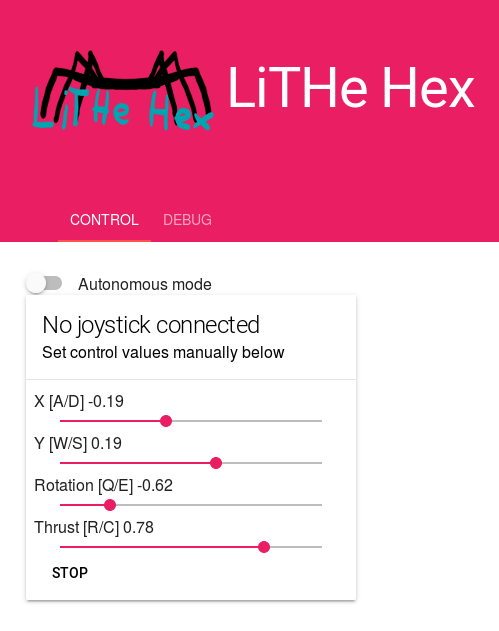
\includegraphics[width=1\linewidth]{images/gui-control.png}
        \caption{Styrning för det manuella läget}
      \end{subfigure}
      \begin{subfigure}{.5\textwidth}
        \centering
		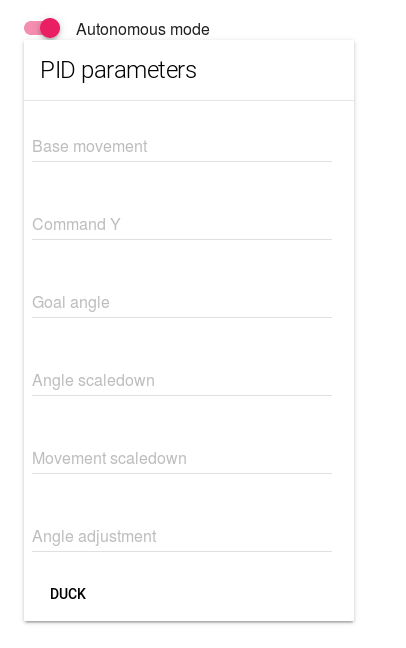
\includegraphics[width=1\linewidth]{images/gui-parameters.png}
		\caption{Parametrar för det autonoma läget}
      \end{subfigure}
      \caption{Det grafiska gränssnittet för control\label{fig:gui-control}}
	\end{figure}
	
	När man har öppnat controlsidan antas det att en joystick är inkopplad i
    datorn. Om det finns en joystick inkopplad så kan man styra roboten med den.
    Om man drar joysticken åt ett håll rör sig roboten i den riktningen, En
    vridning av joysticken kommer göra att roboten vrider sig. På joysticken
    finns också ett gasreglage som styr hur snabbt roboten går och en
    återställningsknapp som gör att roboten återgår till sitt ursprungsläge och
    ställer sig upp igen.

    Om man inte har en joystick finns det olika reglage på skärmen man själv kan
    ändra: X- och Y-led, rotation samt thrust.
	
	Det finns en knapp som heter stop som stoppar roboten. Längst upp finns
    också en knapp för att välja mellan autonomt och manuellt läge. Manuellt
    läge är grundvärden. Se figur \ref{fig:gui-control} för att se hur webbsidan
    ser ut.
	
	\subsection{Debug}\label{gui:debug}
	När man öppnat debug så finns det nio stycken olika grafer som visar olika
    sensordata för roboten vid det här tillfället. Graferna uppdateras tio
    gånger i sekunden för de nya värden som kommer in. Se figur
    \ref{fig:gui-debug} för hur debugsidan ser ut.
	
	\begin{figure}[h]
		\centering
		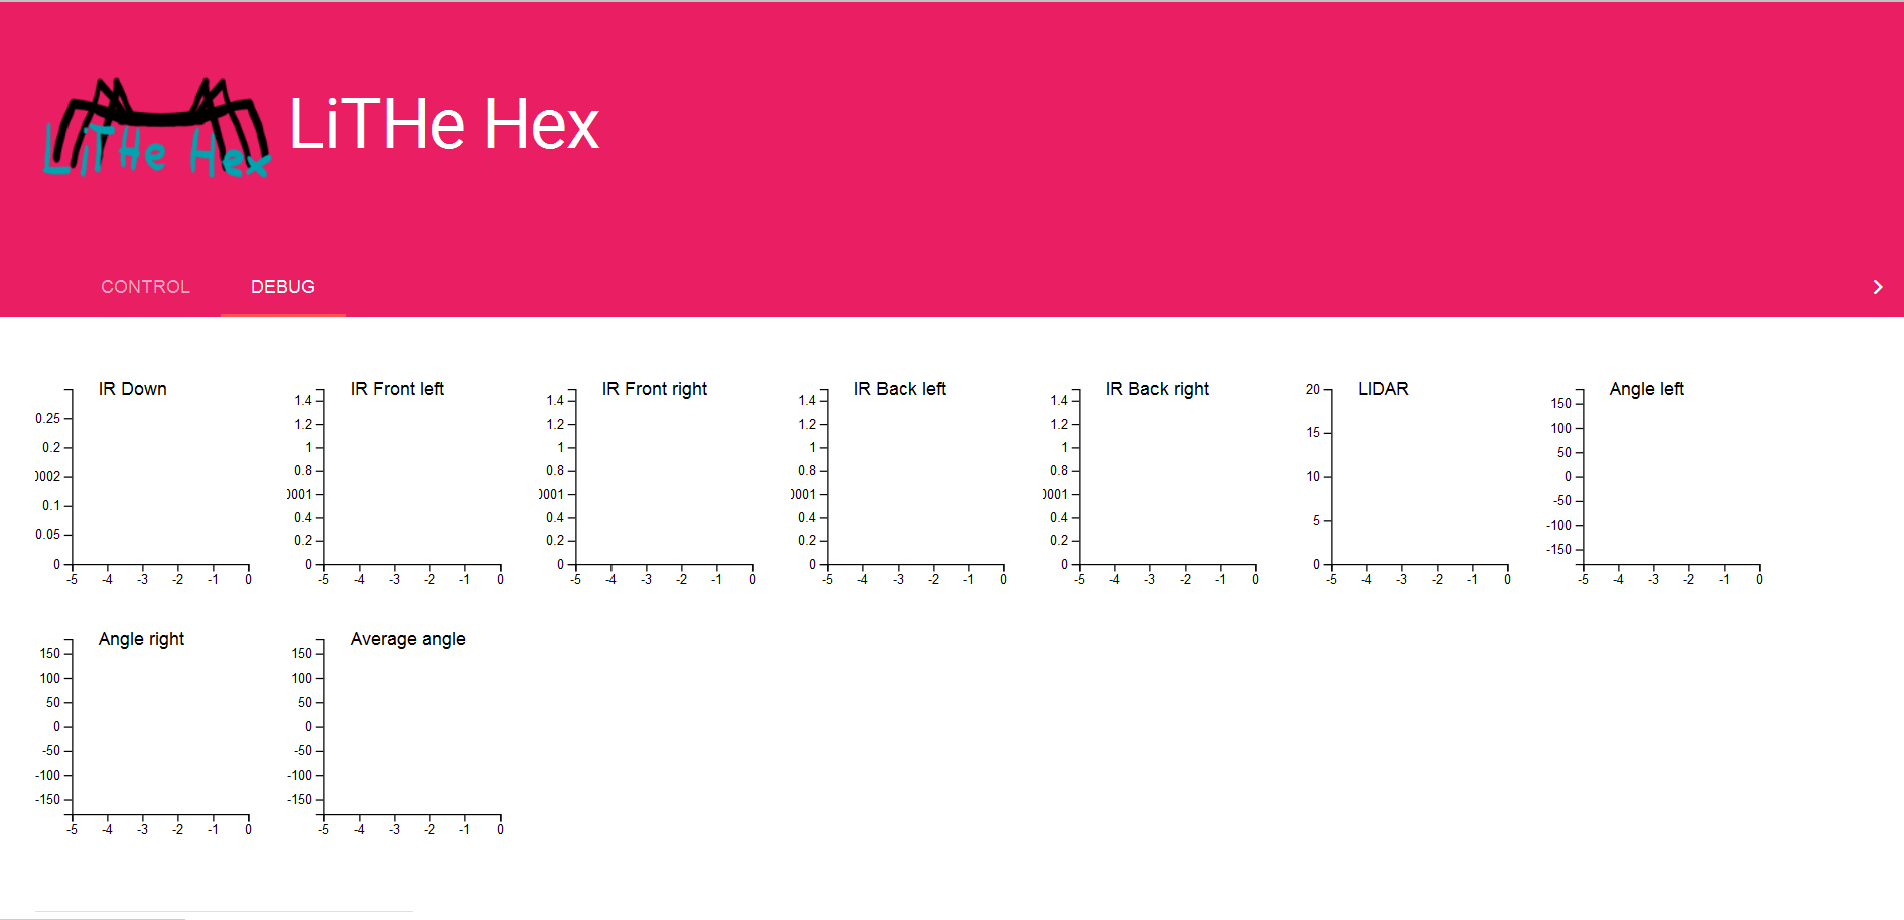
\includegraphics[width=0.5\linewidth]{images/gui-debug.png}
		\caption{Det grafiska gränssnittet för control\label{fig:gui-debug}}
	\end{figure}
	
	% TODO: Ta med om man behöver uppdatera t.ex. phoenix eller liknande?

\end{document}
